\chapter{超导体HfRuP家族中的拓扑态}\label{chap:hfrup}


基于第一性原理计算和实验测量,我们报道了三元相变金属磷化物TT'X (T=Zr, Hf; T'=Ru; X=P, As) 具有拓扑不平庸的性质。这类材料是已知的非中心对称且有较高的转变温度的超导体。在超导转变温度之前,我们发现
HfRuP属于外尔半金属,有12对第II类外尔点;而ZrRuAs,ZrRuP和HfRuAs属于拓扑晶体绝缘体,有平庸的Fu-Kane $\mathbb Z_2$指标,但有非平庸的镜面陈数。这种有两类不同的拓扑态的非中心对称超导体的高质量的单晶样品已经由实验获得,而且超导性也得到实验验证。ZrRuAs比较宽范围的能带结构已经由ARPES确认,并由理论计算重复。与本征的超导性质相结合,这种正常态不平庸的拓扑性可能会在体态和表面态产生非传统的超导性。我们的发现将会激起大量的实验对这类化合物可能的拓扑超导性进行探索。


\section{背景}
    
拓扑绝缘体~\citep{TIreview,qi2011}和拓扑半金属~\citep{Wan2011,xu2011chern,wang2012dirac,wang2013three,weng2015weyl} 由于存在新奇的拓扑态在过去几年受到了极大的关注,例如拓扑绝缘体中自旋-动量锁定的无能隙表面态~\citep{PhysRevLett.106.257004,zhang2013spin}, 和外尔半金属中的负磁阻~\citep{weng2015weyl,huang2015observation,zhang2016signatures}和费米弧态~\citep{xu2016observation,xu2015discovery,wang2016observation2}。这些绝缘体可以由拓扑不变量和拓扑指标来刻画, 如对拓扑绝缘体和拓扑晶体绝缘体分别由Fu-Kane $\mathbb Z_2$ 指标~\citep{Fu2007topo}和镜面陈数~\citep{hsieh2012topological,nie2016band} 来刻画。但是,外尔半金属是有具体的偶然的二度简并点的拓扑金属态,可由三维的外尔方程来描述。由于缺少严格的洛伦兹不变量,第II类外尔半金属会强烈倾斜~\citep{soluyanov2015type},这在高能物理中没有对应。与具有点状体费米面的第I类外尔半金属~\citep{weng2015weyl,huang2015weyl,lv2015experimental,lv2015observation,lv2015observation2,nie2017topological,nie2019magnetic,PhysRevLett.117.236401}相比,第II类外尔半金属~\citep{deng2016experimental,jiang2017signature,tamai2016fermi,liang2016electronic,wang2016mote} 在外尔点既有电子型的口袋,又有空穴型的口袋,这带来了各种各样新奇的物理性质~\citep{kumar2017extremely,shekhar2015extremely}。
    
    
有超导性的拓扑材料是探测拓扑超导(TSC)和马约拉那费米子(Majorana)的理想系统~\citep{yan2013large,wu2015,Schoop2015,chang2016,wang2016spontaneous,xie2017,nie2018}。拓扑狄拉克锥表面态可以与本征的体态超导来诱导产生2D的拓扑超导~\citep{Fu2008superconducting,Fu2010odd,alicea2012new,sato2017topological}。最近,FeTe$_{1-x}$Se$_x$~\citep{wang2015,xu2016}的拓扑表面狄拉克锥态的超导能隙已经由分辨光电子能谱~\citep{Zhang182}和扫描隧道显微镜~\citep{Wang333}实验探测到了。在非中心对称外尔半金属中,3D时间反演对称的拓扑超导可以由具有不同陈数的费米表面中的符号变化的超导性诱导\citep{qi2010,Hosur204}。但是,据我们所知,几乎所有非中心对称的外尔半金属需要外部压力或者掺杂去诱导或者提高超导性\citep{pan2015pressure,kang2015superconductivity,qi2016superconductivity,chen2016superconductivity,li2017concurrence,xu2019topological}。由于缺少合适的候选材料,3D拓扑超导在实验上研究的非常少。因此,高质量的外尔半金属单晶材料的提出和相关的更高的超导转变温度(T$_C$)引起科学家们极大的兴趣。   
    
    
三维相变金属磷化物TT'X (T=Zr, Hf; T'=Ru; X=P, As)是一系列已知的超导体~\citep{barz1980ternary,meisner1983superconductivity}。我们知道,对于这些化合物有三类不同类型的晶体结构\citep{MULLER1983177,meisner1983superconductivity},即Fe$_2$P-类六角结构单晶 (h-相) ,TiNiSi-类正交结构 (o-相) , 和TiFeSi-类正交结构 (o$'$-相) 。在 h- 和 o- 相中发现有超导性,而且一般来说 h- 相的超导转变温度$T_C$比 o- 相更高。在这个工作里,我们仅关注TT'X的 h- 相,这个相表现出相对较高的转变温度$T_C$ (例如,HfRuP的$T_C$为12.7 K \citep{barz1980ternary},ZrRuP为13.3 K,ZrRuAs为12 K \citep{meisner1983superconductivity})。根据第一性原理计算,我们揭示了这些材料在正常状态(T $ _C $以上)的非平庸的拓扑特性。
当忽略自旋轨道耦合(SOC)时,它们在$k_z=0$面内拥有略高于费米能量 (E$_F$) 的两个节点环,每个环在六角布里渊区(BZ)里环绕K点。 在考虑SOC后,他们或者是由于缺少中心反演进入有12对第二类外尔点的外尔半金属相 (例如 HfRuP) , 或者是进入有平庸Fu-Kane $\mathbb Z_2$指标\citep{Fu2007topo}但有非零陈数的拓扑晶体绝缘体相。这些材料中不平庸的电子态
可以激发有关拓扑电子状态与超导性相互作用的大量实验研究的兴趣。
    
    
\section{结果和讨论}
\subsection{计算方法}
本课题采用了基于缀加平面波方法~\citep{paw1,paw2}的VASP软件包 \citep{KRESSE199615,vasp}进行第一性原理计算。采用PBE类型的GGA作为交换关联泛函 \citep{pbe}。平面波截断能设为400 eV。 采用10 $\times$10 $\times$ 16 k网格做自洽计算。采用了实验的晶格常数\citep{Meisner1983,MEISNER1983983}。内部原子位置完全弛豫,直到所有原子受力小于0.01 eV/\AA~[弛豫后的原子位置在表格~\ref{tab:str}]。计算了考虑和不考虑自旋轨道耦合的电子能带结构。拓扑不变量和手性电荷通过Wilson-loop方法计算。采用最局域Wannier函数方法计算了表面态\citep{mlwf}。


\begin{table}[!h]\scriptsize
    \centering
    \bicaption{TT'X的 h- 相(P$\bar 62m$) 化合物的ICSD号,晶格常数($a$和$c$),实验数据和弛豫后的数据。
    三个X原子在原胞中占据1b Wyckoff位置(0, 0, 1/2)和2c Wyckoff 位置(1/3, 2/3, 0)。这里($\alpha,\beta,\gamma$)是以(a, a, c)为单位的分数坐标。~\citep{qian2019npj}
    }
    {The ICSD number, lattice constants ($a$ and $c$), experimental data and relaxed data of the h-phase (P$\bar 62m$) of the TT'X compounds are given. Three X atoms occupy both the 1b Wyckoff (0, 0, 1/2) and the 2c Wyckoff (1/3, 2/3, 0) positions in a unit cell. Here, a fractional position ($\alpha,\beta,\gamma$) is given in units of (a, a, c). ~\citep{qian2019npj}
    }\label{tab:str}
    \begin{tabular} {cccccc}
%    \hline
    \hline
      Compound  & ICSD Number& $a$ (\AA) & $c$ (\AA)  & Experimental data & Relaxed data \\
    \hline
    HfRuP & \#53035\cite{Meisner1983} & 6.414 & 3.753  &  Hf (0.585, 0, 0.5); Ru (0.243, 0, 0) &  Hf ( 0.584, 0, 0.5); Ru (0.245, 0, 0)  \\
%    \hline
    ZrRuP & \#648037\cite{Meisner1983}& 6.459 & 3.778  &  Zr (0.603, 0, 0.5); Ru (0.263, 0, 0) &  Zr ( 0.584, 0, 0.5); Ru (0.243, 0, 0)  \\
%    \hline
    HfRuAs&\#604605\cite{Meisner1983}  &6.568 &3.842   &  Hf (0.584, 0, 0.5); Ru (0.245, 0, 0) &  Hf ( 0.582, 0, 0.5); Ru (0.245, 0, 0)  \\
%    \hline
    ZrRuAs& \#611301\cite{MEISNER1983983} & 6.586 &3.891  &  Zr (0.580, 0, 0.5); Ru (0.250, 0, 0) &  Zr ( 0.582, 0, 0.5); Ru (0.243, 0, 0)  \\
    \hline
%   \hline
    \end{tabular}
\end{table}

\subsection{晶体结构和电子结构}
\begin{figure}[!htbp]
    \centering
    \includegraphics[width=14 cm]{hfrup-fig1.pdf}
    \bicaption{
        TT'X的晶体结构,布里渊区,X射线衍射谱(XRD)和输运性质。(a)晶体结构俯视图:棕色,灰色,绿色分别代表T, T' 和X 原子。
        (b) 晶体的透视图。 
        (c)体布里渊区,(001)-表面布里渊区和(100)-表面布里渊区。此后,(001)[(100) 或(010)] 代表笛卡尔坐标系下表面的法向量。
        (d)和(e)分别为ZrRuAs和HfRuP的索引粉末XRD光谱。红色的星是一小部分杂质。(d)和(e)左边的插图分别是ZrRuAs和HfRuP的单晶样品的照片,右边插图是ZrRuAs和HfRuP在各种磁场下随温度变化的纵向电阻率。 磁场垂直于$ c $轴和电流方向。~\citep{qian2019npj}}
     {The crystal structure, BZs, XRD spectra and transport properties of TT'X.
      ($\bold a$) The top view of the crystal, with brown, gray and green balls representing T, T' and X atoms, respectively.
      ($\bold b$) The perspective view of the crystal. 
      ($\bold c$) The bulk BZ, (001)-surface BZ and (100)-surface BZ. Hereafter, (001) [(100) or (010)] refers to the surface normal vector in terms of the Cartesian coordinates.
      ($\bold d$) and ($\bold e$) Indexed powder XRD spectra of ZrRuAs and HfRuP, respectively. Red stars are small amount of impurities. The left insets of ($\bold d$) and ($\bold e$) are photographs of ZrRuAs and HfRuP single crystals, respectively.  The right insets of them are temperature dependent longitudinal resistivity of ZrRuAs and HfRuP at various magnetic fields. The magnetic fields are perpendicular to $c$ axis and electronic current direction. ~\citep{qian2019npj}
      }
      \label{fig:4-1}
\end{figure}


TT'X的 h- 相空间群是$P\bar 6 2m$ (\#189),层状结构。在六角晶格中每一层被T和X原子或者T'和X原子占据。
所有原子占据在平行于 $ab$- 面的平面内,而且由晶格常数$c$的一半所分开。
三个T'原子(T'$_3$)在 $ab$- 面内形成三角团簇。TT'X的晶体结构如图~\ref{fig:4-1} (a) 和 (b) 所示。T'$_3$团簇和平面结构清晰可见。高对称$\bold{k}$点和表面投影如图~\ref{fig:4-1} (c) 所示。这个结构有两类镜面对称性,$m_z$和$m_x$,这是定义镜面陈数的关键,将在下面讨论。同时,我们也成功生长了单晶样品ZrRuAs和HfRuP,分别展示在图~\ref{fig:4-1} (d) 和 (e) 。 ZrRuP和HfRuP的六角结构通过X射线衍射衍射 (XRD) 得到确认。
ZrRuP和HfRuP的超导性分别由电阻测量(如图~\ref{fig:4-1} (d) 和 (e) 的插入中)和磁化率测量(如图~\ref{hfrup-fig:s6})得到确认。
我们可以看到在温度低于超导相变温度时,两个样品都出现了零电阻现象和迈斯纳效应。


\begin{figure}[!h]
    \centering
    \includegraphics[width=12 cm]{hfrup-figs6.png}
    \bicaption{ (a)ZrRuAs 和(b)HfRuP随温度变化的磁化率曲线。磁场分别垂直于$c$和平行于$c$轴方向施加。~\citep{qian2019npj}}
    {Temperature dependences of magnetic susceptibility of ZrRuAs and HfRuP, respectively. The magnetic field was applied perpendicular and parallel to $c$ axis. ~\citep{qian2019npj}
    }\label{hfrup-fig:s6}
\end{figure}
    

\begin{figure}[!htb]
    \centering
    \includegraphics[width=15 cm]{hfrup-figs1.pdf}
    \bicaption{Ru-基化合物(a-d)不考虑SOC和(e-h)考虑SOC的能带结构。~\citep{qian2019npj}}
    {The band structures  of the Ru-based compounds (a-d) without SOC and (e-h) with SOC. ~\citep{qian2019npj}
    }\label{hfrup-fig:s1}
\end{figure}
    
我们首先检查了没有自旋轨道耦合时候的电子结构,如图~\ref{hfrup-fig:s1}。在这些化合物中,我们主要仔细研究了HfRuP和ZrRuAs,分别作为第II类外尔半金属和拓扑晶体绝缘体相的范例。观察~\ref{fig:4-2} (a) 中HfRuP的能带结构,我们发现在靠近费米能E$_F$除了沿着$M-K$和$K-\Gamma$有能带交叉外,其余$\bold{k}$点有直接的带隙(由浅蓝色标出)。事实上,在这两条线在$k_z = 0$的面内,这个面上有$m_z$对称性。两条交叉能带的$m_z$本征值分别为$\pm 1$。因此这两个交点其实是$m_z$保护的节点环的一部分,节点环围绕$k_z = 0$面内的K点,如图~\ref{fig:4-2} (c) 所示。
这与CaAgAs的情况不同 \citep{yamakage2015line},在那里只有一个$\Gamma$点的节点环。
两个绕着两个K点的节点环也在其他化合物中被发现 (参考ZrRuAs,HfRuAs和ZrRuP的能带结构,如图~\ref{hfrup-fig:s1}) 。
我们可以得出结论,能带反转发生在K点,这可以由拓扑量子化学理论支持~\citep{tqc2017,Vergniory2019}。通过交换在K点 (有小群$D_{3h}$) 上最高价带 ($\Gamma_4$) 和最低导带的表示 ($\Gamma_1$) ,占据态能带变成是平庸的,可分解为基本能带表示(EBR)的线性组合~\citep{tqc2017}。

\begin{figure}[!htbp]
\centering
\includegraphics[width=\textwidth]{hfrup-fig2.pdf}
\bicaption{
        在不考虑(a)和考虑(b)SOC时HfRuP的电子能带结构。其中K点选定的能带的不可约表示也标记在图中。
        (c)展示没有SOC时,$k_z=0$面内的节点线。有SOC时,在第一布里渊区里位于$k_z=0$面上方的外尔点标记为 ``+"(+1)和``o"(-1)。
        这里,$\bf a$*,$\bf b$*,和$\bf c$* 是倒空间原胞基矢。
         (d) 穿过外尔点(c)中W1的电子沿着$k_z$方向的能带色散。
         (e)穿过外尔点(c)中W1的电子沿着P-Q方向的能带色散。W1,P和Q的分数坐标分别是$(0.2761 , -0.4654, 0.02439)$和$(0.2603 , -0.4603, 0.02439)$,和$(0.2919 , -0.4705, 0.02439)$。此后,给出的$k$点的位置以($\bf a$*, $\bf b$*, $\bf c$*)为单位。
        ZrRuAs的角分辨光电子谱(ARPES)(f)和曲率强度(g) 展示了沿着H-K-H的能带结构。为了进行比较,图(g) 将沿H-K-H计算的能带结构叠加在实验数据上。(h-i)和(f-g)一样,但是是沿着L-M-L方向的。~\citep{qian2019npj}
        }
        {
        The electronic band structures of HfRuP without (a) and with (b) SOC.
        The irreducible representations of selected bands at K point are indicated.
        (c) The nodal lines are presented in the $k_z=0$ plane without SOC.
        With SOC, the WPs above the $k_z=0$ plane are labeled as ``+"(+1) and ``o"(-1) in the first BZ.
        Here, $\bf a$*, $\bf b$*, and $\bf c$* are the reciprocal primitive vectors.
        (d) The $k_z$ dispersion of the electronic bands through the WP W1 shown in (c).
        (e) The dispersion of the WP W1 along the line P-Q shown in (c).
        The fractional coordinates of W1, P and Q are $(0.2761 , -0.4654, 0.02439)$, $(0.2603 , -0.4603, 0.02439)$, and $(0.2919 , -0.4705, 0.02439)$. Hereafter, the positions of $k$-points are given in units of ($\bf a$*, $\bf b$*, $\bf c$*).
        ARPES spectrum (f) and curvature intensity (g) plots of ZrRuAs, showing band structure along H-K-H. For comparison, the calculated band structure along H-K-H is superposed on the experimental data in (g). (h-i) are the same as (f-g), but along L-M-L. ~\citep{qian2019npj}}
\label{fig:4-2}
\end{figure}
    
在考虑自旋轨道耦合之后,能带结构变化不大,但是由于缺少中心反演对称性,能带发生劈裂。
为了确认密度泛函理论 (DFT) 得到的能带结构的可靠性,我们对ZrRuAs进行了ARPES测量,展示在图~\ref{fig:4-2} (f) - (i) 。沿着H-K-H和L-M-L观察到的谱与DFT计算结果 (图~\ref{fig:4-2} (g) 和 (i) 中红色的线) 吻合的非常好,特别是对于低能的能带。我们可以很清楚的看到,K点的能带比M点能带更低。另外,两条简并的节点环由于SOC而打开。二维时间反演不变的平面 (如 $k_y = 0$和$k_z = 0$等面) 完全打开能隙,使得$\mathbb Z_2$不变量可以很好的定义。在CaAgAs中,绕着$\Gamma$点的单个的节点环由于有限的SOC强度使得$k_y = 0$ (或者$k_z = 0$)面是$\mathbb Z_2$不平庸的。但是这和两个K点有两个节点环的ZrRuAs情况不同。对于这些化合物,$k_y = 0$和$k_z = 0$两个面的 $\mathbb Z_2$不变量仍然是平庸的。注意$k_y = 0$即使是没有SOC也是打开能隙的,而且在所有时间反演不变的平面都没有能隙闭合的点。为了确定$\mathbb Z_2$不变量是平庸的,在 $k_y = 0$ ($k_z = 0$) 面,我们计算了$k_z$- 指向的 ($k_y$- 指向的) Wilson loop的瓦尼尔心作为$k_x$的函数 (称为Wilson-loop bands) 。ZrRuAs的结果如图~\ref{hfrup-fig:s2} (a) 和 (b) ,在$k_y = 0$ 面和$k_z = 0$面$\mathbb Z_2$不变量是平庸的。其余的四个时间反演不变的平面的$\mathbb Z_2$不变量细节也展示在图~\ref{hfrup-fig:s2}。类似地,所有这些化合物的Fu-Kane $\mathbb Z_2$指标~\citep{Fu2007topo} 为 (0;000) 。

\begin{figure}[!htb]
    \centering
    \includegraphics[width=1\textwidth]{hfrup-figs2z2}
    \bicaption{ZrRuAs四个时间反演不变平面内占据态能带的Wannier心的演化。~\citep{qian2019npj}}{
    The flow of WCCs for all occupied energy bands in four TRI planes of ZrRuAs. ~\citep{qian2019npj}
    }\label{hfrup-fig:s2}
\end{figure}
    
我们进一步发现这些材料的对称性指标~\citep{nc_ashvin,song2017,Jorrit2017,zhang2019,wanxg2019} 为$\mathbb Z_{3m,0}=1$和$\mathbb Z_{3m,\pi}=0$,揭示了SOC能隙如图~\ref{fig:4-2} (b) 的拓扑本质。
    
      
\subsection{镜面陈数和外尔点}
\begin{figure}[!htbp]
    \centering
    \includegraphics[width=0.8\textwidth]{hfrup-fig3.pdf}
    \bicaption
    {时间反演不变平面上的瓦尼尔电荷中心(WCC)。
    (a)和(b)分别为$k_y = 0$ 和$k_z = 0$面作为$k_x$函数的$k_z$- 指向和 $k_y$- 指向的Wilson loops。
    (c)和(d)分别为HfRuP 和 ZrRuAs在$k_x = 0$面内作为$k_y$函数的$k_z$ - 指向的Wilson loops。
    红色和蓝色的圈分别代表有镜面本征值为$+i$和$-i$的能带的WCC流。水平的虚线代表参考线。~\citep{qian2019npj}
    }
    {The WCCs of TRI planes.
    (a) and (b) The WCCs of the $k_z$-directed and $k_y$-directed Wilson loops as a function of $k_x$ for the $k_y = 0$ and $k_z = 0$ planes, respectively.
    (c) and (d) The WCCs of the $k_z$-directed Wilson loops as a function of $k_y$ in the $k_x = 0$ plane of HfRuP and ZrRuAs, respectively.
    Red and blue circles represent the flow of the WCCs for the bands with mirror $+i$ and $-i$ eigenvalues, respectively.
    The horizontal dashed lines are reference lines. ~\citep{qian2019npj}}
    \label{fig:4-3}
\end{figure}    
    
    
由于镜面对称性的出现,只要镜面上的能带完全打开能隙,镜面陈数就可以很好的定义。因为时间反演对称操作和镜面对称操作对易,陈数满足$C_i =  -C_{-i}$,下标$\pm i$代表有SOC时的镜面本征值。镜面陈数可以定义为$C_m = (C_{+i}-C_{-i})/2$。众所周知,在半个镜面上,这可以进一步推导为$\chi_{+i}-\chi_{-i}$,其中$\chi_{+i(-i)}$可以很容易的通过画Wilson-loop bands,通过在 $+i~(-i)$子空间数水平参考线[如图~\ref{fig:4-3} (c) 和 (d) 中的虚线]与斜率为正的能带相交的次数减去与斜率为负的能带相交的次数。对于$k_x = 0$平面,ZrRuAs的计算结果如图~\ref{fig:4-3} (d) 。ZrRuAs的$k_z$ = 0的镜面陈数$C_{m_z}$ 计算结果为$-2$,而$k_z =\pi$的镜面陈数为0。这个家族的所有化合物的镜面陈数情况如图~\ref{hfrup-fig:s3}。

\begin{figure}[!htb]
    \centering
    \includegraphics[width=1\textwidth]{hfrup-figs3}
    \bicaption{ 当考虑自旋轨道耦合时,Ru-基化合物在(a-d)$k_x=0$ 和(e-h)$k_z=0$ 面的镜面陈数。红色的圈代表镜面本征值为$+i$的能带的WCCs流,蓝色的圈代表镜面本征值为$-i$的能带的WCCs流。
    在(e-h)中,黑色虚线是任意选择的参考线,目的是为了看参考线和Wilson-loop正负斜率的能带交叉的次数。(e)中放大的插图显示了连接方式的细节。~\citep{qian2019npj}}
    {
    The mirror Chern numbers of Ru-based compounds  for (a-d) $k_x=0$ and (e-h) $k_z=0$ planes when SOC is considered. Red circles represent the flow of the WCCs for bands with mirror $+i$  eigenvalue and blue circles for bands with mirror $-i$  eigenvalue.
    The black dashed line in (e-h) is an arbitrarily selected reference line for the purpose of counting the number of crossing times between the reference line and the Wilson-loop bands with positive and negative slopes. The zoom-in inset of (e) shows the connective pattern clearly. ~\citep{qian2019npj}
    }\label{hfrup-fig:s3}
\end{figure}
    
    
中心对称性的破缺允许系统中出现外尔点。非零的镜面陈数$C_{m_z} =-2$ 表明在$ k_z = 0 $平面中存在一些规范奇异的线穿过\citep{bernevig2015s},这必须在三维布里渊区的某些外尔点上终止。我们系统的计算表明,根据$k_x=0$面上的镜面陈数$C_{m_x}$不同,这些化合物可以分为两类:i)一类有为零的镜面陈数 $C_{m_x} =0$,这类有12对第II类外尔点,称为外尔半金属相; ii) 另一类有非零的镜面陈数 $C_{m_x} =2$,这一类没有外尔点,称之为拓扑晶体绝缘体相。HfRuP在 $k_x=0$面的瓦尼尔电荷中心如图~\ref{fig:4-3} (c) ,镜面陈数 $C_{m_x}$为0。不能完全补偿的$m_z$和$m_x$ 面的镜面陈数表明系统中存在外尔点,而且在这个材料中确实发现了外尔点,这和外尔半金属相相吻合。但是,对于ZrRuAs,HfRuAs和ZrRuP,$C_{m_x}$计算表明是$2$,如图\ref{fig:4-3} (d) 和图~\ref{hfrup-fig:s3}。由于镜面陈数完全补偿,所以这些系统中不存在外尔点。事实上,在这几个材料中我们也确实没有发现外尔点存在。

通过检查能隙和相关的拓扑单极电荷,我们发现从每个节点环产生6对外尔点。因此在第一布里渊区共有12对外尔点如图~\ref{fig:4-2} (c) 。他们处于同样的能量,因为他们由时间反演对称性和晶体对称性$D_{3h}$ (包括12个对称操作)相联系。在图~\ref{fig:4-2} (c) 中,由虚线包围的外尔点W1的坐标是[0.2761$\bf a$*, $-$0.4654$\bf b$*, 0.02439$\bf c$*]。 从W1沿着$k_z$- 方向 [图~\ref{fig:4-2}(d)]和P-Q 方向[图~\ref{fig:4-2}(e)]的色散,我们可以知道它属于第II类外尔点~\citep{xu2015},它的能量(E$_W$)在费米能E$_F$以上28 meV (即E$_W$-E$_F= 28$ meV),非常接近费米能。拓扑单极电荷可以由包裹外尔点的闭合流型上计算Wilson-loop的方法获得。外尔点W1的单极电荷是+1。$k_z = 0$面以上所有外尔点的分布如图~\ref{fig:4-2} (c) ,``+(o)" 代表拓扑电荷$+1(-1)$,而在$k_z = 0$以下的外尔点由于$m_z$对称性有相反的单极电荷,如图~\ref{fig:4-2} (c) 。
    
    
\subsection{表面态上的费米弧}
\begin{figure}[!htbp]
    \centering
    \includegraphics[angle=270,width=14 cm]{hfrup-fig4.pdf}
    \bicaption{
    HfRuP的表面谱。(001)- 表面(a),(100)- 表面(b)和(010)- 表面(c) 能量为$E-E_W=0$ meV的表面谱。
    外尔点的投影用菱形或``x''符号标记。~\citep{qian2019npj}}
    {
    The surface spectra of HfRuP. The (001)-surface (a), (100)-surface (c) and (010)-surface (c) energy contours with $E-E_W=0$ meV.
    The projections of the WPs are indicated by diamonds or ``x" symbols. ~\citep{qian2019npj}
    }
    \label{fig:4-4}
\end{figure}    

\begin{figure}[!h]
    \centering
    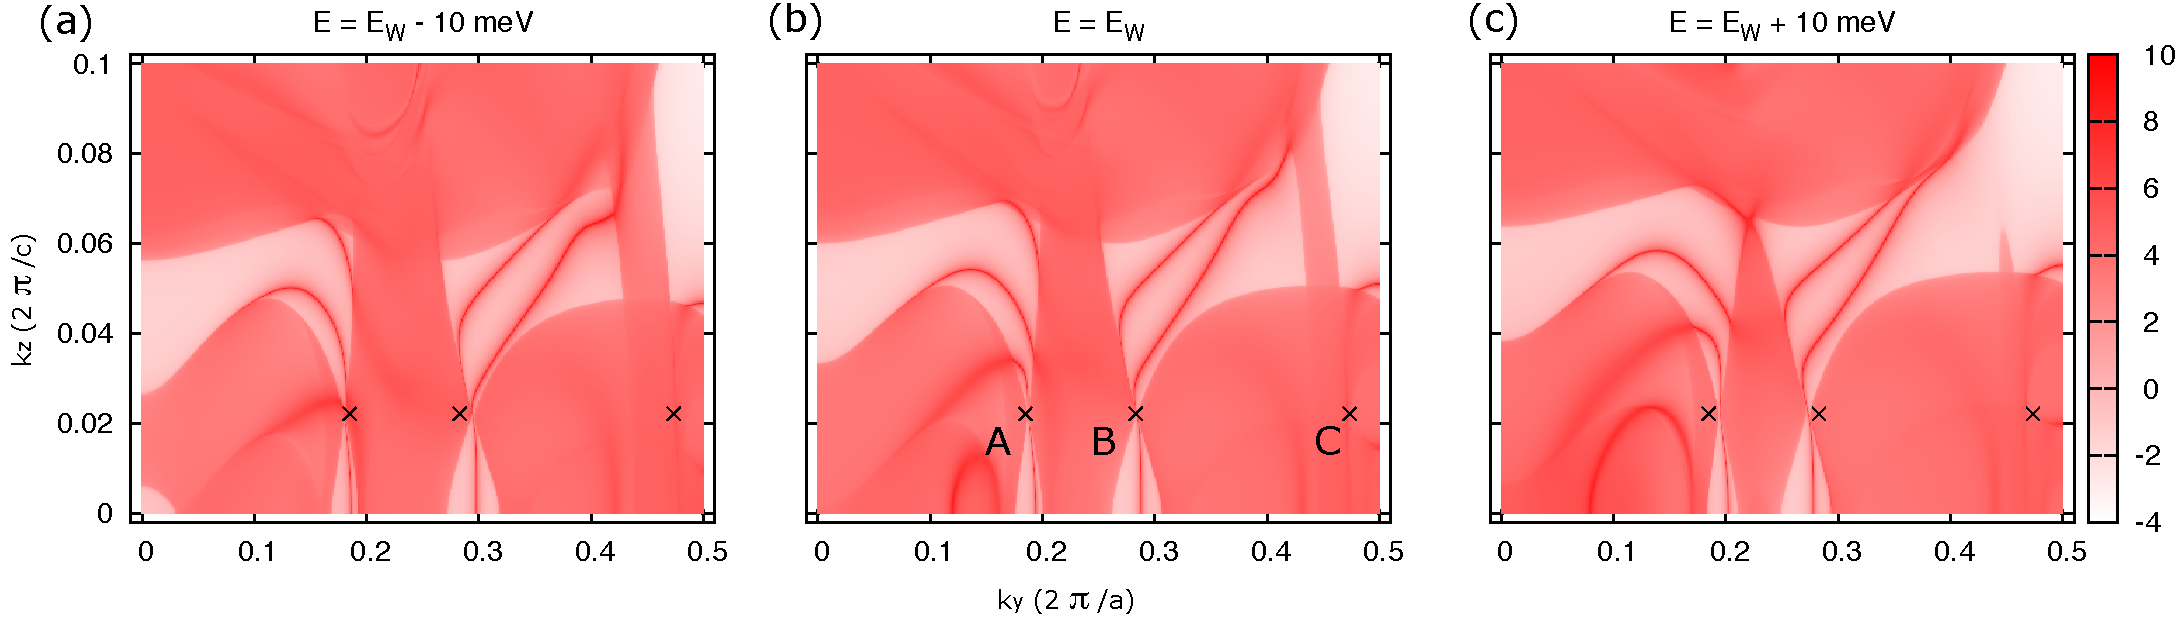
\includegraphics[width=14 cm]{hfrup-figs4}
    %\includegraphics[width=16 cm]{figs3}
    \bicaption{不同等能面外尔点的投影。E$_W$是外尔点所处的能量位置。~\citep{qian2019npj}}
    {
    The different energy contours with the projections of WPs.
    E$_W$ is the energy level of the WPs. ~\citep{qian2019npj}
    }\label{hfrup-fig:s4}
\end{figure}
  
在外尔半金属中,我们期望出现连接两个手性相反的外尔点的投影的表面费米弧。为了这个目的,基于格林函数的方法\citep{Sancho_1985},我们计算了半无限大的最局域化的瓦尼尔函数的表面态。首先,在图~\ref{fig:4-4} (a) 中给出了HfRuP的(001)表面能量为$E-E_W=0$ meV的表面态。因为在 (001) 表面两个手性相反的外尔点投影到同一个点,所以不能保证从投影的点出发有拓扑的费米弧表面态。但是,我们发现有两条平庸的arc态从每个外尔点的投影出来:一个arc穿过$k_x = 0$的线;另一个穿过布里渊区边界,(即, $\bar K- \bar M$线)。其次,计算的(100)等能面如图~\ref{fig:4-4} (b) 所示。因为他们是第II类外尔点,外尔点应该位于电子口袋和空穴口袋相接触的点。我们也确实看到了在两个口袋接触点的地方有外尔点的投影A和B。我们看到了两条表面费米弧(用虚线标记)连接投影点 (即,A和B) 。对于投影点C,很难看到任何从它出发的表面态,因为它没有投影到一个合适的表面上。最后,计算的 (010) 表面的等能面如图~\ref{fig:4-4} (c) ,其中相同手性的外尔点投影到一起。只要电子/空穴口袋 (包裹外尔点的投影) 彼此分开,我们就可以期望出现两条拓扑的费米弧态。但是不幸的是,金属型的体态在很大的范围内都有投影,这使得费米弧态无法看到。我们在(100)表面寻找费米弧的ARPES实验仍在进行中。
  
这些外尔点是第二类外尔点,为了解释这一点,我们画了(001)表面在能量稍微低于或者高于E$_{W}$的常数能量的等能面的表面态展示在图~\ref{hfrup-fig:s4}。
从低一点的能量 (E=E$_W$-10 meV) 到更高一点能量 (E=E$_W$+10 meV) , 我们可以清楚的看到外尔点的投影 (例如 A点 或者 B点) 从一个口袋变到另一个口袋。从投影C点, 很难看到类似点演化过程,因为没有投影到合适的方向。
%%%%  

\subsection{新奇的拓扑超导态}
凭借固有的超导性,由于在正常状态下波函数具有非平凡的拓扑结构,拓扑材料是实现拓扑超导的有前途的平台。例如,表面狄拉克费米子甚至可以在$ s $波配对状态下实现二维拓扑超导\citep{Fu2008superconducting,wang2015}。而且,正常态费米面的拓扑会直接影响拓扑超导性。在三维,在时间反演不变的超导体中整数的拓扑量子数由配对序参量的符号和在费米面上的贝利相位规范场的第一陈数决定~\citep{qi2011}。超导体中的外尔半金属相有来源于外尔点的不平庸的拓扑。HfRuP的外尔半金属相提供了两个关键要素:非平庸的费米面和超导电性,可以作为实现3D时间反演不变的拓扑超导的良好平台。除此之外,之前的工作~\citep{shingo2015,ueno2013}报道了不平庸的镜面陈数可以产生Cd$_3$As$_2$和SrRuO$_4$中的多重Majorana费米子。这些化合物中的拓扑晶体绝缘体相也是寻找拓扑晶体超导体的极有希望的候选者。
    
\section{结论}
基于DFT计算,我们发现TT'X的 h- 相在没有SOC的能带结构有两个节点环,这与CaAgAs不同。在考虑SOC后,这些化合物或者进入有12对第II类外尔点的外尔半金属相,或者进入有非零陈数的拓扑晶体绝缘体相。两个不同相的单晶样品已经成功生长出来。他们的超导性和电子能带结构通过我们电阻测量,磁化率,和ARPES测量的分别得到验证。这一系列Ru基化合物都是单晶化合物,在T$_C$以下有超导性,在T$_C$ 以上有拓扑性。这项工作将促进对超导性与外尔或非平庸镜面陈数态之间相互作用的实验研究。
 
